% (c) 2014 Michiel Appelman
\section{Introduction} % (fold)
\label{sec:introduction}
Network operators today use \acp{nms} to get control over their devices and services that they deploy. These systems have been customized to their needs and in general perform their functionalities adequately. However, operators run into obstacles when trying to expand their business portfolio by adding new services. Which will potentially require
\begin{inparaenum}[\itshape a\upshape)]
	\item new \ac{api} calls to be implemented between their OSS and \ac{nms}, 
	\item their \ac{nms} to be able to cope with potentially new protocols, and
	\item added expertise by engineers to define the possible feature interactions and restrictions of these protocols \cite{programmability-answer}. 
\end{inparaenum}
When these obstacles are eventually overcome the setup that will result from this implementation will be relatively static, since any change to it will require the whole process to be repeated.

%Until recently this limitation didn't distress operators as their networks were in fact primarily static. But with increasing demand for services requiring for example mobility and short-term virtual networks, these limitations start to become a tangible problem for operators. By solving the complexity of implementing new services or features for them, they will be able shorten their time to market, save on networking expertise and be more adaptive to changes in these services. %referenties

To manage resources efficiently in a carrier network operators have been using \acp{vpn} between customers. By differentiating traffic between \acp{vpn} they can control their traffic flow at a granular level. However, the set of interactions between different protocols and management interfaces to them are complex. The provisioning of \acp{vpn} requires expertise and a significant amount of changes to those protocols. Until recently operators were not concerned by this rigidness as their networks were in fact primarily static. However, the demand for application specific networks is growing and operators are looking for a more flexible approach in the form of \acp{dvpn}. \acp{dvpn} are private networks over which end-users can communicate, deployed by their common \ac{sp}. They differ from normal \acp{vpn} in the sense that they are relatively short-lived. Using \acp{dvpn}, \acp{sp} can react more swiftly to customer requests to configure, adjust or tear down their \acp{vpn}. However, due to the aforementioned complexity \acp{dvpn} services have not been implemented on a large scale.

A potential candidate to solve the complexity of implementing \acp{dvpn} is OpenFlow \cite{openflow} and \ac{sdn}. \ac{sdn} is a relatively new architecture to allow for the programmability of networks. The architecture is not standardized but a generalized structure has been given in the OpenDaylight project \cite{opendaylight} which also includes OpenFlow as can been seen in Figure~\ref{fig:opendaylight}. OpenFlow is a lower level and increasingly supported \ac{api} protocol towards networking devices. Implementing the \ac{sdn} architecture promises
\begin{inparaenum}[\itshape a\upshape)]
	\item CAPEX savings due to hardware being more generic and flexible,
	\item OPEX savings because of the integration of \acp{nms} and the control interface of the devices, thereby increasing automation, and
	\item increased network agility by using the open interfaces to program network devices directly \cite{packet-circuit}.
	\end{inparaenum} 

\begin{figure}[!h]
	\centering
	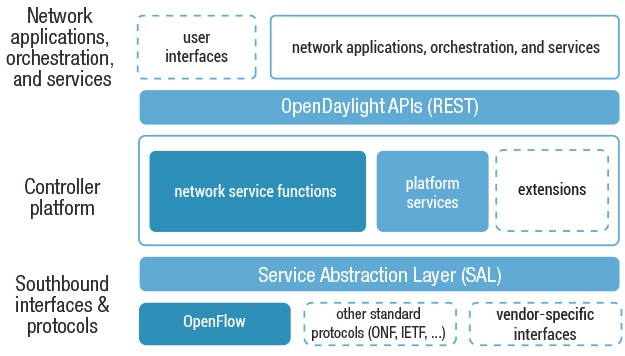
\includegraphics[width=10cm]{./includes/opendaylight.jpg}
	\caption{The proposed OpenDaylight architecture.}
	\label{fig:opendaylight}
\end{figure}

	\subsection{Research Question} % (fold)
	\label{sub:research_question}
	It is unclear however if a real-world OpenFlow and \ac{sdn} implementation will actually provide any simplicity, additional flexibility or cost savings when compared to contemporary technologies \cite{programmability-answer}. And so the question arises: \textsl{``How much can operators benefit from using OpenFlow when implementing \aclp{dvpn}?''} 
	This requires research into whether \acp{dvpn} can be provisioned by current technologies and how this can be implemented in the network. Additionally, we will research the possibility of implementing \acp{dvpn} using OpenFlow. And finally we will attempt to prove the hypothesis that OpenFlow will reduce the complexity in the architecture of the management systems and the network as a whole.

	% subsection research_question (end)

	\subsection{Scope} % (fold)
	\label{sub:scope}
	The focus will primarily be on deploying \acp{ppvpn} at Layer 2 of the \acs{osi}-model between end-users. We haven chosen to do so because these Ethernet \acp{vpn} are characterized by their transparency to the end-user, who will be placed in a single broadcast domain with its peers and can thus communicate directly without configuring any sort of routing.
	
	Previous research in \cite{net-prog-vpn} has proposed a very specific implementation for programmable networks to deploy on-demand \acp{vpn} but it predates the OpenFlow specification, and also omits a comparison with how this would look using contemporary technologies.

	% subsection scope (end)

	\subsection{Approach} % (fold)
	\label{sub:approach}
	In the Section~\ref{sec:dvpns} we will define the conceptual design of \acp{dvpn}. This will result in a list of required features for the technologies to provide such a service. Section~\ref{sec:implementation} will list the technologies available and will additionally determine their usability for implementing \acp{dvpn} when taking into account the requirements set forth in Section~\ref{sec:dvpns}. In Section~\ref{sec:results} we will distill the advantages and limitations of the different implementations and substantiate how the compare to each other. Finally, Section~\ref{sec:conclusion} summarizes the results and provides a discussion and future work on this subject.

	% subsection approach (end)

% section introduction (end)